\documentclass{article}

\usepackage{color}
\usepackage{cite}
\usepackage{float}
\usepackage{graphicx}
\usepackage{pgfgantt}

\linespread{1.3}

\title{Telemetry-based Optimisation for User Training in Racing Simulators \\ Progress Report}

\author{Francois Buhagiar}
\date{2015}

\begin{document}

\pagenumbering{roman} 

\maketitle
\newpage
\tableofcontents

\pagenumbering{arabic} 
\setcounter{page}{1}

\newpage
\begin{abstract}
\end{abstract}

\newpage
\section{Introduction}
The gamification of areas of activity such as marketing, problem solving and education \cite{michael2005serious} has validated the use of serious games beyond their initial military use in training strategic skills \cite{djaouti2011classifying}.  Serious games simulate real-world processes designed for the purpose of solving a problem, making their main purpose that of training or educating users. Their popularity has been steadily increasing, as has their adoption, with military \cite{djaouti2011classifying} and emergency service providers (e.g. firefighters \cite{michael2005serious}) employing them to train for specific scenarios that might be encountered on the respective jobs. Motorsports cover a broad range of activities and vehicles, and as with all major forms of sporting activities, require training and dedication, with a pedagogic aspect arising in rote learning and mentoring by experts. The arenas in which motorport events take places are called circuits; there is a large selection of the latter, ranging from purposely built race tracks to public roads to natural formations such as hills and quarries. There is also a diverse selection of vehicles that take part in motorsports, with the greatest demarcation existing between motorbikes and cars. The focus of this dissertation is that of unifying serious games and motorsport racing; specifically, it will try to show whether a serious game is a powerful enough pedagogical tool that can be used to tangibly improve the performance of race drivers. The scope of the project is limited to four-wheeled cars racing on purposely-built confined circuits with a smooth tarmac surface.  

\section{Motivation}
The training process for race drivers has stabilised during the last decade, with rote learning playing a very important part. Starting at an early age, a driver would compete in lower leagues, such as go karting, and undergo training that is mostly founded on trial and error. A mentor, or coach, would correct obvious mistakes and suggest ways for improvement based on experiential knowledge and related literature. The extensive hours of practice serve to hone the skills of a driver and help in the acquisition of the same experiential knowledge of the mentor. Such learning methodology is very resource consuming in that it requires both time and money; often it is geographically-constrained as well, where no suitable training track is available in the locality of the driver. Although simulators, such as those employed by professional racing teams, have helped mitigating traveling and car setup times, they are inadequate for use in more amateurish environments due to cost and logistical problems: setting up such a simulator requires adequate space seldom available to everyone. Democratising the learning process such that proper car control and racing techniques can be mastered by a larger demographic an important motivation behind this work.

\section{Why the problem is non-trivial}
The problem at hand is best described as an optimisation problem. Telemetry data provided by the car instrumentation system can be analysed to help identify driving patterns, specifically car-handling mistakes. The identification of these behaviours, which traditionally employs pattern recognition techniques, represents a challenge in itself. Behaviour recognition is key to providing corrective measures in order to improve the driving performance of a given user. In particular, it is the starting point in building a model which maps telemetry data to corrective measures for presentation to the user in real-time and deferred fashion, where even the visualisation of feedback is critical to the success of such a system.

\section{Background Work}

\subsection{Motorsport racing}

In sports individuals or groups compete to be first to achieve a particular objective. In the case of circuit motorsport races, in which motorised vehicles go round a course. Each racing discipline or series has its own rules. However, at the core, all disciplines participants aim to complete a full lap of the circuit in the least amount of time. Some disciplines focus on achieving one fast lap, such as time trials, while others focus on achieving the least amount of time across a fixed amount of laps, such as FIA's Formula 1 series. This dissertation will focus on confined car racing taking place on smooth asphalt surfaces in purpose built race tracks. 

A race driver needs to figure out how to go round a piece of asphalt in the minimum amount of time \cite{GoingFaster}. In order to do so, he or she needs to develop techniques for more advanced vehicle control. One such technique is that of mastering the race line, which is considered the the fundamental skill a race driver must understand and master before moving on to anything else \cite{GoingFaster}. The racing line is the best path through a circuit, it is the one which takes the least time while keeping the higher average speed \cite{beckman1991physics}. The trickiest part of the racing line to master is that of a corner. This is split into two parts, identifying the line which should be taken and staying on the line. The first part refers to being able to visualise the racing line while the later refers to actually being able to control the car so that it stays on the line. 

\subsection{Video games and Serious Games}

Baranowski et al \cite{yuserious} define games as a physical or mental contest with a goal or objective, played according to a framework, or rule, that determines what a player can or cannot do inside a game world. The definition covers the setup of a game, while a physical or mental contest, played according to specific rules, with the goal of amusing or rewarding the participant the reward aspect of games.

Video games are built on top of these core values with the addition of having the game world confined to some sort of digital medium. The first video game was created by William Higinbotham; it was a tennis game to be played on a television set\cite{stanton2015brief}. From the early days of video games, their main aim was always to provide some degree of entertainment. The entertainment value is achieved in various ways depending on the gaming platform, game genre and the target audience. Modern video games are simply made up of three fundamental components: story, art and software \cite{zyda2005visual}.

Moving on to serious games this type of games are considered a mix of simulation and game to improve eduction \cite{abt1970}. The idea behind a serious game is to connect a serious purpose to knowledge and technologies from the video game industry\cite{michael2005serious}. The boundaries of serious games are debated, mostly due to the fact that serious games attract multiple domains making it hard to come up with a common boundary. However, the common denominator across all domains seems to be serious game designers use people's interest in video games to capture their attention for a variety of purposes that go beyond pure entertainment\cite{djaouti2011classifying}.

The main contrast between video games and serious games is the use of pedagogic activities which aim to educate or instruct knowledge or skill \cite{zyda2005visual} in serious games as opposed to the pure leisurely aspects of the video game. Pedagogy is given preference over the amusement value which in some cases might not be found in serious games \cite{zyda2005visual}.

\subsection{Sim Racing as a Serious Game}

Simulation racing games (sim racing) such as Asseto Corsa \cite{aqqalla1} and Project CARS \cite{aqqalla2}, which are off-the-shelf products, provide a sim racing experience within budget for the average video game consumer. The aim with such games is to replicate real life cars, race car dynamics and track locations to amuse and entertain the player. The challenge aspect is achieved by pitting the user against other computer drivers known as AI players, or in multiplayer online races, which are played against other human players. In some cases, a user can compete against oneself by taking on a ghost - a recording of the player's best lap for a particular track. Sim racing the definition of what a video game is however, they miss the pedagogy activities which would qualify them as serious games. Most of the modern sim racing games do aid the player to improve by means of implementing aids. Such aids might include showing the racing line while also highlighting the braking and acceleration points. Other aids include anti lock brakes, traction control and stability control, these are implemented in a passive way. With the exception of the racing line, the player is not told when and what is being done wrong. This results in users having to figure out their own mistakes by means of practicing without any guidance or feedback from with the game. This final year project aims to implement a module which is plugged into an off the shelf racing simulator which. This module trains users by letting them know what is being done wrong, when it's being done wrong and most importantly how to avoid making the same mistake.

\section{Aims and objectives}

The aim of this project is that applying serious games in the training of motorsports race drivers; in particular, it aims at testing the hypothesis significant improvement in a driver's lap times can be achieved via a pedagogic feedback system employed to teach the driver and help him or her learn specific racing techniques.

\begin{itemize}
  \item Identify a suitable off-the-shelf race driving simulator \\
  	The simulator will be chosen according to a number of criteria such as simulation realism, visual fidelity and system extensibility.

  \item Identify telemetry information for analysis and feedback system \\
  	The telemetry information provided by the simulator will be scrutinised and a subset identified; this subset will be used in the acquisition component of the feedback and analysis system to assess player performance.

  \item Research, design and develop the rule-based analysis and feedback system \\
  	A rule-based analysis system is developed which takes telemetry data as input and outputs possible corrections for improving lap times. The outputs are selectively sorted and filtered in order to present the user with the most effective corrections (greater return on investment per applied correction).

  \item Design user study to test principal hypothesis.
\end{itemize}

\section{Methods and technologies used or planned}

Two components are being designed, the first being a simulation component which will be assembled out of consumer available sim racing rig hardware. The second component is the software aspect of the project. This component is in turn subdivided into smaller modules, one of which is the telemetry module which handles reading the telemetry provided by a racing simulator. As \ref{fig:SystemComponentArchitecture} demonstrates, the telemetry modules connects to the game, parses the data and encodes it into a format which can be easily worked with by subsequent feedback module before relaying back to the game with the UI rendered feedback.

\begin{figure}[!htb]
	\centering
	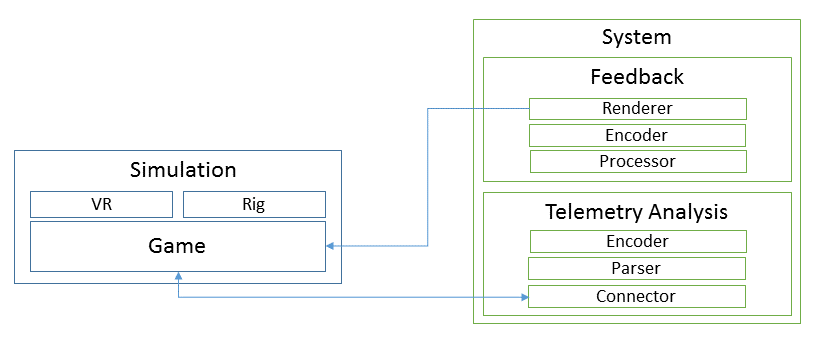
\includegraphics[height=5cm]{SystemArc}
	\caption{System Component Architecture}
	\label{fig:SystemComponentArchitecture}
\end{figure}

Earlier in this report it was discussed the importance for a race driver to adhere to the racing line. In order to reassure how well a user is adhering to the racing line the system must measure for every telemetry data point, which is the nearest racing line's data point and how far is it. The searching for the nearest data point is handled by a quad tree data structure containing all the racing line's data points. The distance is calculated using basic 2d geometry functions. \ref{fig:QuadTree} illustrates a quad tree generated from a specific racing line. 

\begin{figure}[!htb]
	\centering
	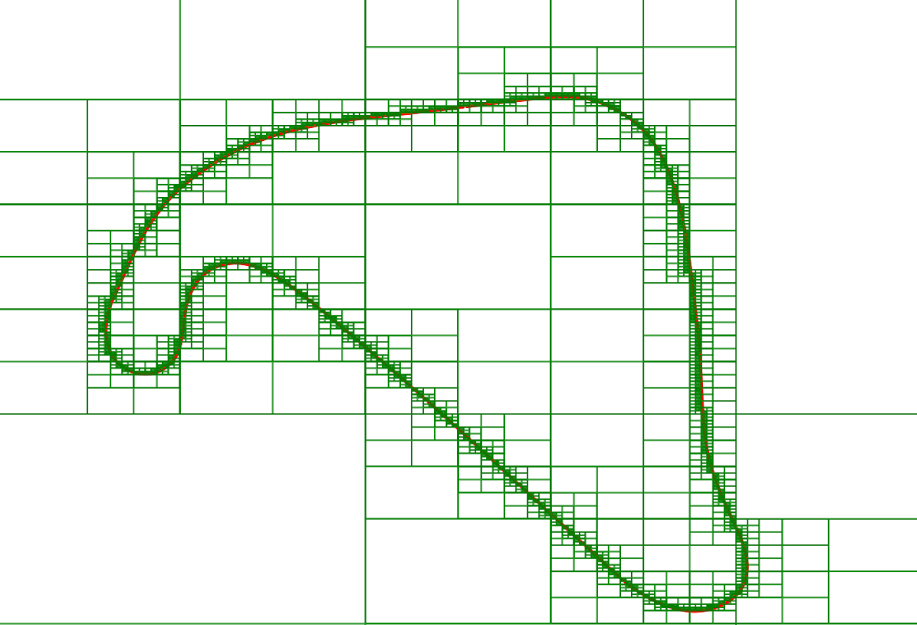
\includegraphics[height=5cm]{QuadTree}
	\caption{Quad tree visual representation}
	\label{fig:QuadTree}
\end{figure}

This project relies heavily on hardware and software components from other third parties. The user study will required a sim racing rig, this is to be made of a mid range sim racing Logitech G25 steering wheel, pedals and shifter in conjunction with a real racing seat and an Oculus Rift virtual reality headset. This hardware choose has been influenced by costs, ease of sourcing, ease of setup and the value the components add to the user study, as individually and collectively. Various racing games have been looked into, iRacing, Project Cars, rFactor and Asseto Corsa are the main ones. Although the implementations differ, all mentioned games do provided the same basic feature required by this project, however, Asseto Corso has been chosen for its ease of integrability, support and documentation. \ref{fig:ProofOfConcept} is a screen shot taken from Assesto corsa with a proof of concept of the system overplayed on top. The overlay is displayed while a user is playing the game, and it is split into two areas. On the left, a map of the circuit is shown with a red circle denoting the car geographical location and in yellow text the distance from the racing line is also shown. On the right side the user is being shown, telemetry values which can let an experienced driver now if corrections are required to the racing style.

\begin{figure}[!htb]
	\centering
	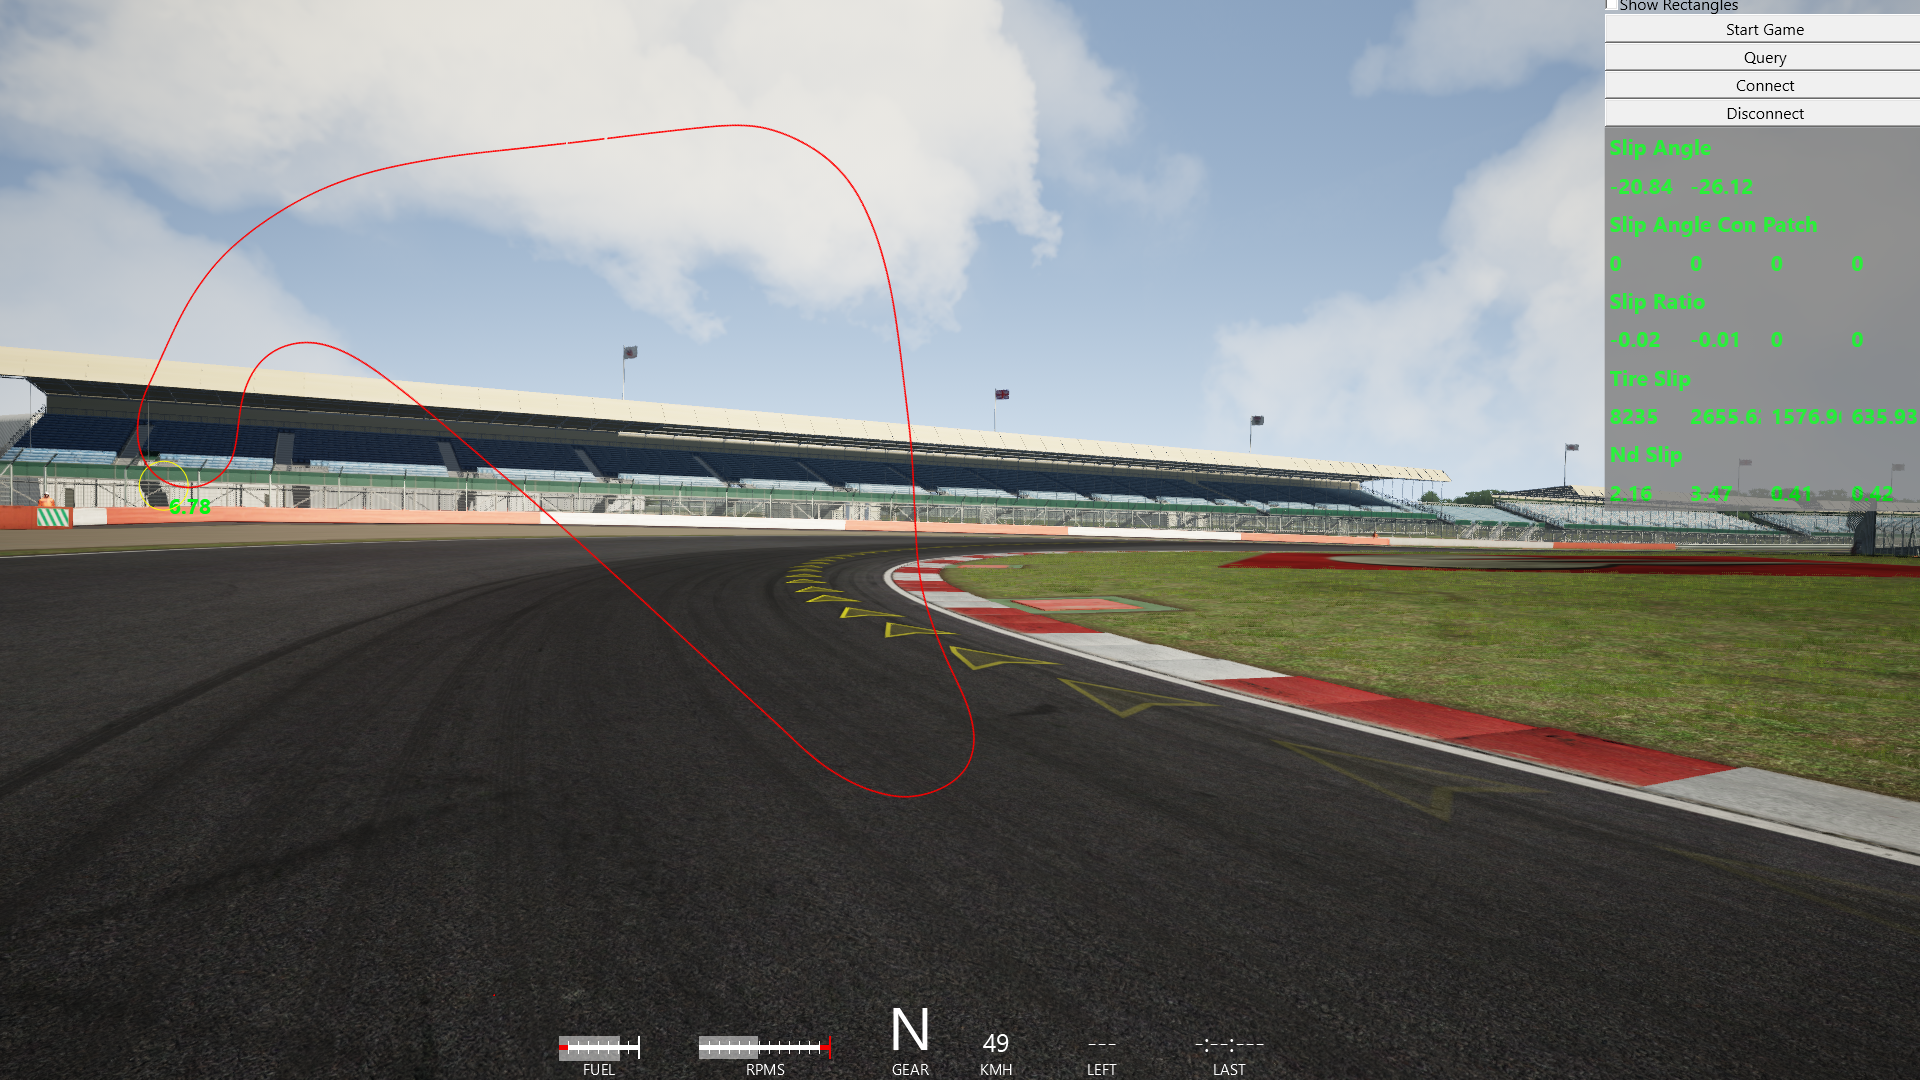
\includegraphics[height=5cm]{Proofofconcept}
	\caption{Proof of concept}
	\label{fig:ProofOfConcept}
\end{figure}

Moving on from the proof of concept the system needs to provide more concrete feedback and better visually represent said feedback. The feedback will be improved by means of fuzzy logic which is to determine what the user can improve in terms of racing by analysing multiple data points. More importantly fuzzy logic will output the degree of gain the user will get from each minor improvement from which the system will be able to better choose which correction the user should be suggested. Lastly, data visualisation will also be looked into as the telemetry data which are shown in \ref{fig:ProofOfConcept} are not easy to understand at a glance, the system needs to present the mistakes and corrections to the user in a away which can be easily understood. 

\section{Evaluation strategy}

A user study is to be carried out to address the project's hypothesis which is asking whether or not users can improve their racing skills by using the suggested setup. The evaluation aspects to be examined are the ease of understanding and carrying out the suggested feedback, the rate of learning of test subjects, and the effectiveness of the feedback given.

\subsection{Experiment setup}
A simulation rig is to be setup in order to provide a sense of realism to the users which will be participating in the tests. The rig will be made of a racing wheel which provides force feedback, a three pedal set and a racing seat. Virtual reality will also be integrated into the system as to provide better sense of immersion. A race track and car will be preselected. This selection will be made based on ease of track layout and ease of car handling characteristics. 

\subsection{User study}
Users are to be divided into two groups at random. One group of users will be asked to drive around the track without having any feedback provided from the system. This will evaluate how much a user can improve on their own. While the second group will also be asked to drive around, but this time the system will provide feedback on where and how the user can improve. A set of questions will be asked to the user once the test is complete. The questioner is meant to collect data on the users' racing experience prior to taking the test. Telemetry data will also be collected for both groups. Statistical analysis will be carried to determine if lap times do improve. From this analysis 

\section{Deliverables}
A report based on the user study will be produced. The report will contain a summary for each experiment, the summary will contain the test subjects' answers to the questioner, telemetry data and feedback given by the system, From these summaries a another report is to be created containing the finds from the study. The main aim of the report is to outline the validation process used to accept or reject the hypothesis put forward by this project.

\section{Work Plan}

\begin{figure}[!htb]
	\centering
	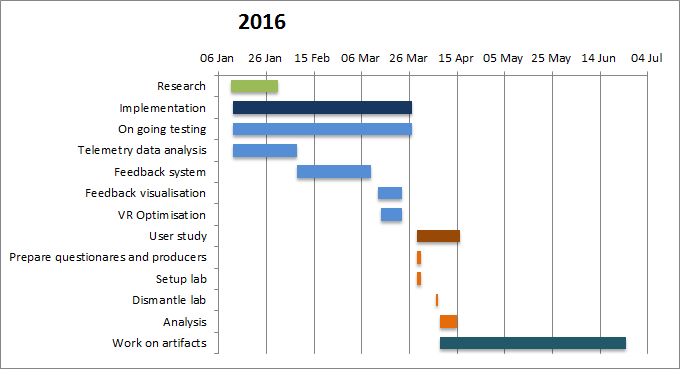
\includegraphics[height=8cm]{TimeLine}
	\caption{Time line}
	\label{fig:Time Line}
\end{figure}

\newpage
\bibliography{citeations}{}
\bibliographystyle{plain}

\end{document}